\section{Results}
\label{sec:Results}

\begin{figure*}
    \centering
    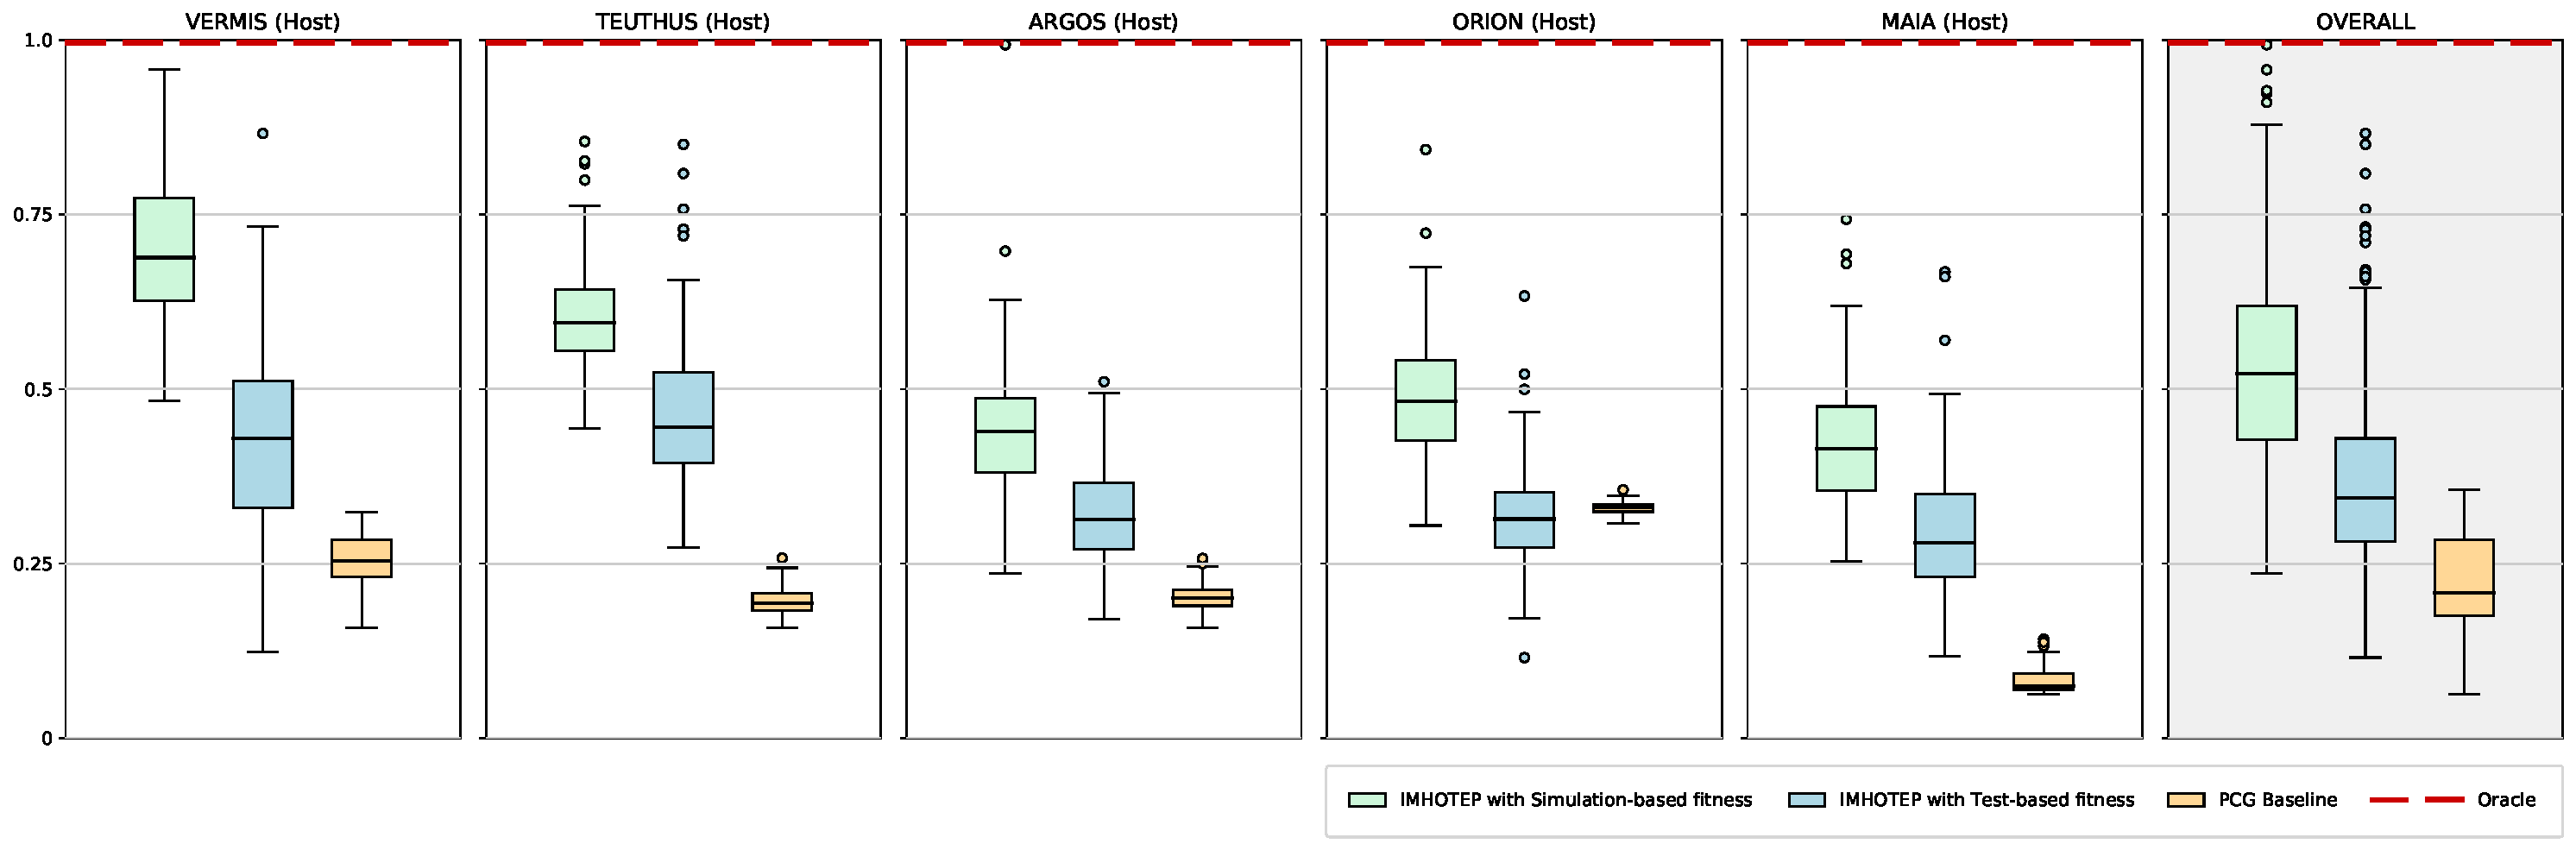
\includegraphics[width=\textwidth]{Figures/Imhotep_with_legend_and_oracle_average-v4.pdf}
    \caption{Results}
    \label{fig:results}
\end{figure*}

Figure \ref{fig:results} shows the results of the evaluation execution of our approach when using the two objective functions (Simulation-Based and Test-Based) from \ApproachName{} and the PCG Baseline. The executions are grouped by each host (boss of \CaseStudy{}) that has been used in our experiment (Vermis, Teuthus, Argos, Orion, and Maia). The last column, with shaded background, shows the average of all of the host for each objective function and the baseline. In addition, the oracle indicates the value obtained by the human-generated final boss models that were obtained from the \CaseStudy{}. 

Each boxplot is generated from the results of each host' obtained from the transplantation of each of the 5 hosts with each of the 129 organs. Therefore, each boxplot represents 645 values of a specific host-organ transplantation in a final boss model. Figure \ref{fig:results} shows in each column how the quality values obtained for each of the three strategies studied in our evaluation differ from the values for the models generated by the developers, which are represented by the horizontal red dashed lines that cross each host column. The boxplots that are closer to the horizontal lines are more similar in quality to the models produced by the developers. Additionally, the use of boxplots allows for the representation of the different results for the strategies used.

\todo{Analysis of the results. Simulation has the best results, test also better than baseline...}


\begin{table*}[t!]
    \caption{Mean Values and Standard Deviations}
    \centering
    \resizebox{\textwidth}{!}{%
    \begin{tabular}{llllllll}
    \toprule
    &\multicolumn{1}{c}{Vermis}
    &\multicolumn{1}{c}{Teuthus}
    &\multicolumn{1}{c}{Argos}
    &\multicolumn{1}{c}{Orion}
    &\multicolumn{1}{c}{Maia}
    &\multicolumn{1}{c}{Overall}
    \\ \midrule
    Simulation
    & 0.699 $\pm$ 0.105 & 0.607 $\pm$ 0.074 & 0.439 $\pm$ 0.093 & 0.488 $\pm$ 0.087 & 0.430 $\pm$ 0.121 & 0.533 $\pm$ 0.142       
    \\
    Test
    & 0.424 $\pm$ 0.130 & 0.463 $\pm$ 0.105 & 0.321 $\pm$ 0.069 & 0.314 $\pm$ 0.068 & 0.295 $\pm$ 0.093 & 0.363 $\pm$ 0.117        
    \\
    Baseline
    & 0.254 $\pm$ 0.033 & 0.195 $\pm$ 0.018 & 0.201 $\pm$ 0.018 & 0.329 $\pm$ 0.008 & 0.084 $\pm$ 0.018 & 0.213 $\pm$ 0.083
    \\ \midrule     
\end{tabular}
}

\label{tab:results}
\end{table*}

\begin{table*}[t!]
    \caption{Max and Min values.}
    \centering
    \resizebox{\textwidth}{!}{%
    \begin{tabular}{lllllllllllll}
    \toprule
    & \multicolumn{2}{c}{Vermis}
    & \multicolumn{2}{c}{Teuthus}
    & \multicolumn{2}{c}{Argos}
    & \multicolumn{2}{c}{Orion}
    & \multicolumn{2}{c}{Maia}
    & \multicolumn{2}{c}{Overall}
    \\ \midrule
    \multicolumn{1}{c}{} 
    & \multicolumn{1}{c}{Max} & \multicolumn{1}{c}{Min} 
    & \multicolumn{1}{c}{Max} & \multicolumn{1}{c}{Min} 
    & \multicolumn{1}{c}{Max} & \multicolumn{1}{c}{Min}
    & \multicolumn{1}{c}{Max} & \multicolumn{1}{c}{Min} 
    & \multicolumn{1}{c}{Max} & \multicolumn{1}{c}{Min} 
    & \multicolumn{1}{c}{Max} & \multicolumn{1}{c}{Min} 
    \\
    Simulation & 1.042 & 0.482   & 0.854 & 0.443   & 0.992 & 0.235   & 0.842 & 0.304   & 1.285 & 0.253   & 1.285 & 0.235                          
    \\
    Test & 0.866 & 0.123   & 0.850 & 0.273   & 0.510 & 0.170   & 0.633 & 0.115   & 0.667 & 0.117   & 0.866 & 0.115   
    \\
    Baseline & 0.323 & 0.157   & 0.257 & 0.158   & 0.257 & 0.157   & 0.355 & 0.307   & 0.141 & 0.063    & 0.355 & 0.063
    \\ \midrule                     
\end{tabular}
}

\label{tab:maxmin}
\end{table*}